\documentclass[11pt]{article}
\usepackage[margin=1in]{geometry}
\usepackage{amsmath,amssymb,amsthm,mathtools}
\usepackage{graphicx}
\usepackage{microtype}
\usepackage[hidelinks]{hyperref}

\newcommand{\C}{\mathbb C}
\newcommand{\Dens}{\mathcal D}
\newcommand{\MD}{M_D}
\newcommand{\tr}{\operatorname{tr}}
\newcommand{\rank}{\operatorname{rank}}
\newcommand{\ip}[2]{\langle #1,#2\rangle}
\newtheorem{theorem}{Theorem}
\newtheorem{corollary}{Corollary}

\title{Uncountably many commutant classes of extreme points\\
in a \(D\)-majorization set}
\author{Candidate counterexample for arXiv:2004.05613}
\date{11 August 2026}

\begin{document}
\maketitle

\begin{center}
\fbox{\parbox{0.91\textwidth}{
\textbf{Status: candidate counterexample/full negative answer, likely valid.}
For every nonscalar full-rank density matrix \(D\), a pure state \(A\) can be
chosen so that \(M_D(A)\) is the entire state space.  Modulo unitaries
commuting with \(D\), its extreme points form a positive-dimensional simplex
and hence have uncountably many equivalence classes.}}
\end{center}

\section{Source and open question}

The source is Frederik vom Ende, \emph{Strict Positivity and
\(D\)-Majorization}, arXiv:2004.05613, subsequently published in
\emph{Linear and Multilinear Algebra} 70:19 (2022), 4023--4048 \cite{vomEnde}.
For a positive definite matrix \(D\), let
\[
 Q_D(n)=\{T:M_n(\C)\to M_n(\C):T\text{ is completely positive and
 trace preserving, }T(D)=D\}.
\]
The source writes \(X\prec_D A\) when \(X=T(A)\) for some
\(T\in Q_D(n)\), and
\[
 M_D(A)=\{T(A):T\in Q_D(n)\}.
\]

In Section 5, pages 20--21, the source observes that conjugation by a unitary
commuting with \(D\) preserves the extreme points of \(M_D(A)\).  It then asks
whether factoring out this unitary equivalence leaves only finitely many
extreme points (meaning finitely many equivalence classes).

\begin{figure}[ht]
\centering
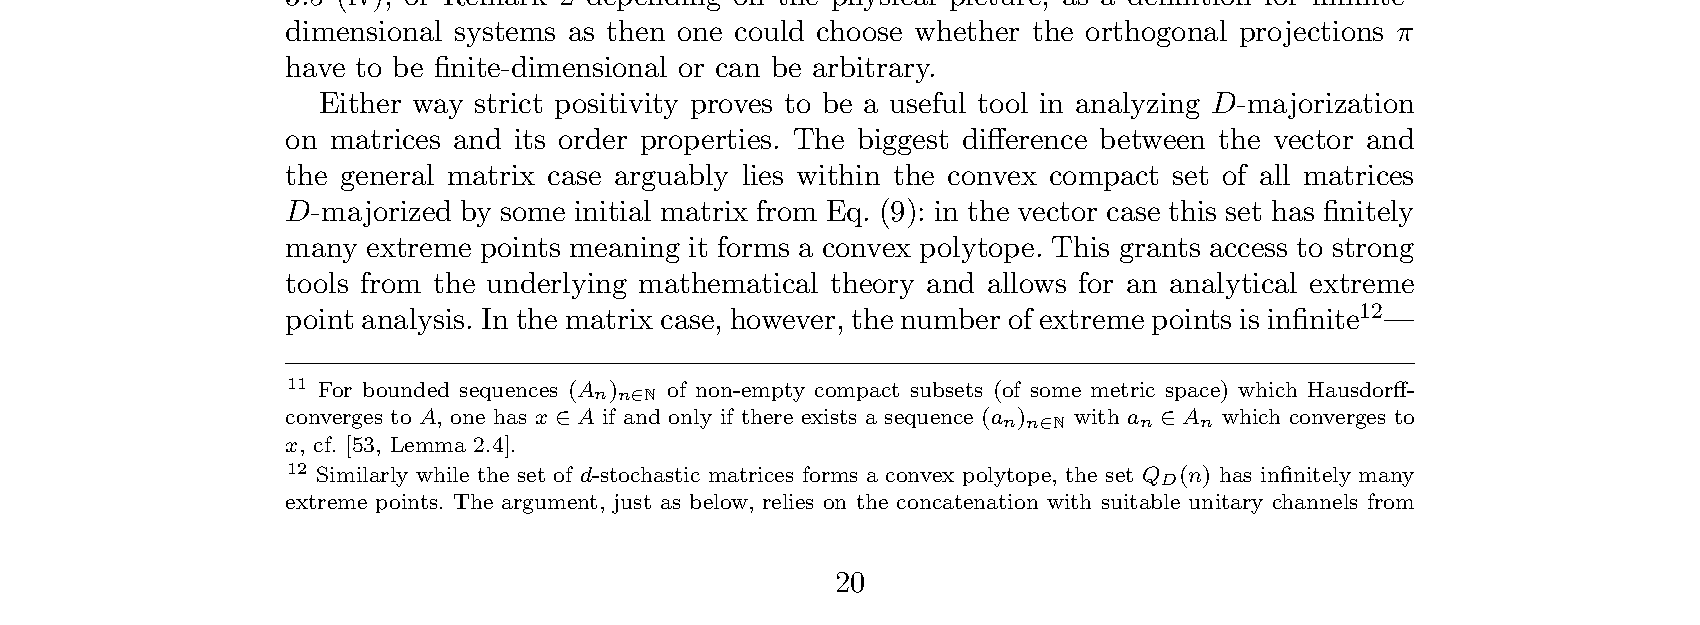
\includegraphics[width=\textwidth]{figures/open_problem_crop_page20.png}
\vspace{0.35em}
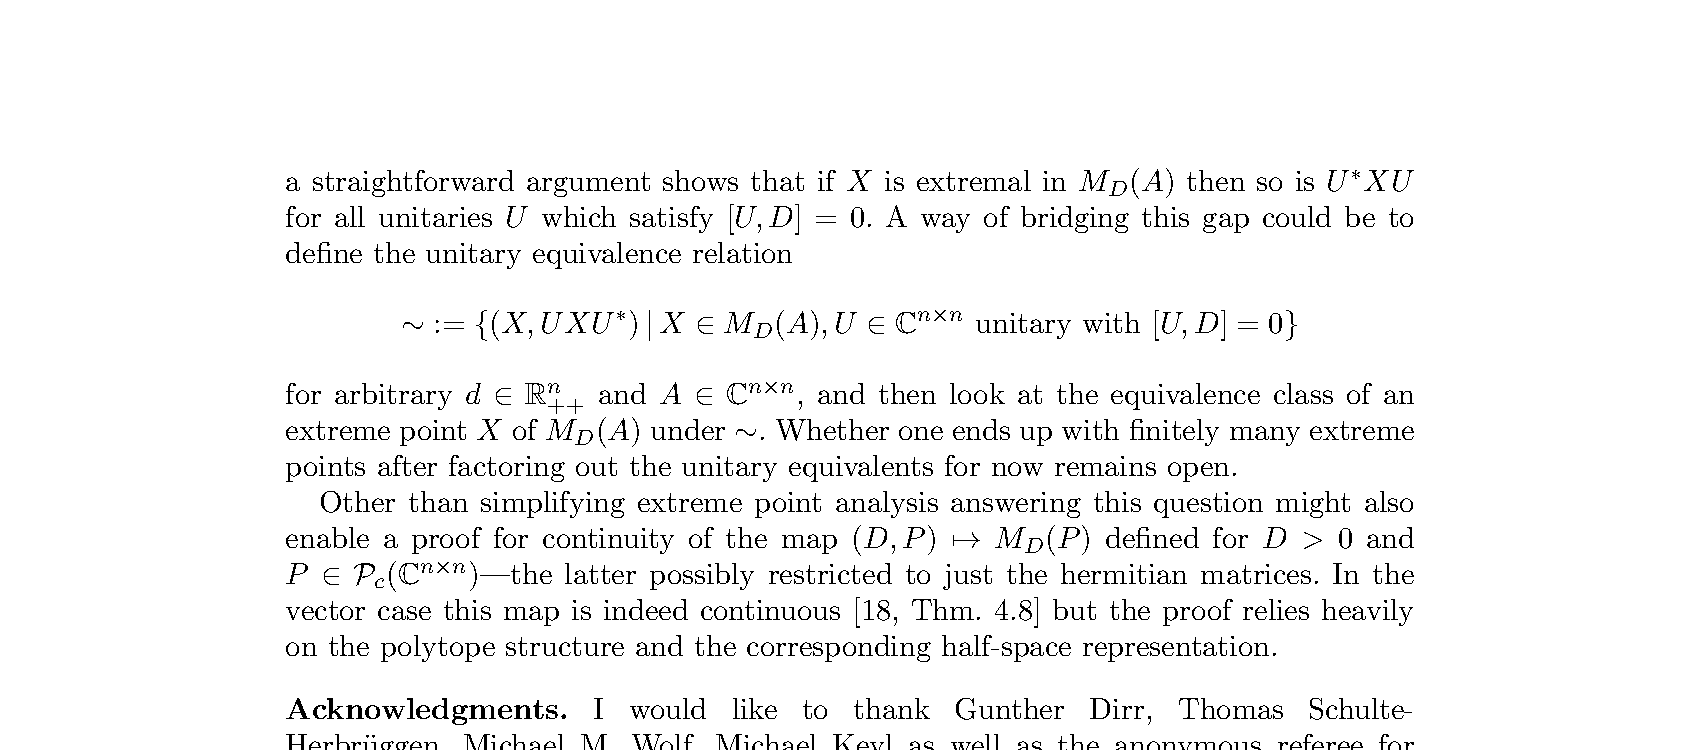
\includegraphics[width=\textwidth]{figures/open_problem_crop_page21.png}
\caption{The concluding discussion and open finiteness question on pages
20--21 of the source PDF.}
\label{fig:question}
\end{figure}

\section{Proof intuition}

Choose \(A\) to be a pure state in a minimum-eigenvalue eigenspace of \(D\).
For every desired output state \(\rho\), the minimum-eigenvalue inequality
makes \(D-d\rho\) positive.  This produces an explicit
measure-and-prepare channel that fixes \(D\) and sends \(A\) to \(\rho\).
Thus \(M_D(A)\) is not merely a complicated convex body: it is the whole
state space.

Its extreme points are the pure states.  A unitary commuting with \(D\)
acts independently inside the distinct spectral subspaces of \(D\), so its
orbit remembers exactly how much squared norm a pure vector has in each such
subspace.  These weights fill a simplex.  When \(D\) is nonscalar the simplex
has positive dimension, giving uncountably many inequivalent extreme points.

\section{Counterexample and exact quotient}

Write \(\Dens_n=\{\rho\in M_n(\C):\rho\succeq0,\ \tr\rho=1\}\).

\begin{theorem}\label{thm:main}
Let \(D\in\Dens_n\) be positive definite and nonscalar, with \(n\ge2\).
Choose a unit eigenvector \(e\) for \(d=\lambda_{\min}(D)\), and put
\(A=|e\rangle\langle e|\).  Then
\[
 M_D(A)=\Dens_n.
\]
If \(D=\sum_{j=1}^r\lambda_jP_j\) is its spectral decomposition over the
distinct eigenvalues, then the extreme points of \(M_D(A)\), modulo
conjugation by unitaries commuting with \(D\), are in bijection with
\[
 \Delta_{r-1}=\left\{(w_1,\ldots,w_r):w_j\ge0,
 \ \sum_{j=1}^r w_j=1\right\}.
\]
In particular, there are uncountably many equivalence classes.
\end{theorem}

\begin{proof}
Fix an arbitrary state \(\rho\in\Dens_n\).  Since \(D\succeq dI\) and
every density matrix satisfies \(\rho\preceq I\),
\begin{equation}\label{eq:positive}
 D-d\rho=(D-dI)+d(I-\rho)\succeq0.
\end{equation}
Also \(0<d<1\), and hence
\[
 \tau:=\frac{D-d\rho}{1-d}
\]
is a density matrix.

Extend \(e=e_1\) to an orthonormal eigenbasis
\(e_1,\ldots,e_n\) of \(D\), and define
\begin{equation}\label{eq:channel}
 T_\rho(X)=\langle e_1,Xe_1\rangle\rho
 +\sum_{k=2}^n\langle e_k,Xe_k\rangle\tau.
\end{equation}
This is a measure-and-prepare channel, hence completely positive.  For
completeness, diagonalizing each prepared state produces Kraus operators
\(\sqrt{s_{k\ell}}|v_{k\ell}\rangle\langle e_k|\); their adjoint products
sum to \(I\), so \(T_\rho\) is trace preserving.  Moreover,
\[
 T_\rho(A)=\rho,
 \qquad
 T_\rho(D)=d\rho+(1-d)\tau=D.
\]
Thus \(\rho\in M_D(A)\).  Since a channel maps a state to a state, the
reverse inclusion \(M_D(A)\subseteq\Dens_n\) is automatic.  This proves
\(M_D(A)=\Dens_n\).

The extreme points of \(\Dens_n\) are exactly the rank-one projections.
Indeed, a state of rank at least two can be perturbed by opposite small
traceless diagonal perturbations inside its support, while any convex
decomposition of a rank-one state forces both summands to have the same
one-dimensional support.

Represent an extreme point as \(E_\psi=|\psi\rangle\langle\psi|\), with
\(\|\psi\|=1\), and define its spectral weight vector
\[
 w(\psi)=\bigl(\|P_1\psi\|^2,\ldots,\|P_r\psi\|^2\bigr)\in\Delta_{r-1}.
\]
If \(U\) commutes with \(D\), then \(U\) preserves each spectral subspace,
so \(w(U\psi)=w(\psi)\).  Conversely, suppose
\(w(\psi)=w(\varphi)\).  On each \(P_j\C^n\), choose a unitary \(U_j\)
sending \(P_j\psi\) to \(P_j\varphi\) (with an arbitrary choice when both
vectors vanish).  Then \(U=\bigoplus_jU_j\) commutes with \(D\) and satisfies
\(U\psi=\varphi\).  Hence \(E_\psi\) and \(E_\varphi\) are equivalent if
and only if their weight vectors agree.

Every point of \(\Delta_{r-1}\) is realized by choosing unit vectors
\(u_j\in P_j\C^n\) and setting \(\psi=\sum_j\sqrt{w_j}u_j\).  The quotient
is therefore exactly \(\Delta_{r-1}\).  Nonscalarity gives \(r\ge2\), so
this simplex, and hence the set of equivalence classes, is uncountable.
\end{proof}

\begin{corollary}[Explicit qubit counterexample]\label{cor:qubit}
Let
\[
 D=\begin{pmatrix}1/3&0\\0&2/3\end{pmatrix},
 \qquad
 A=\begin{pmatrix}1&0\\0&0\end{pmatrix}.
\]
Then \(M_D(A)=\Dens_2\), and the extreme points
\[
 \left|\sqrt t\,e_1+\sqrt{1-t}\,e_2\right\rangle
 \left\langle\sqrt t\,e_1+\sqrt{1-t}\,e_2\right|,
 \qquad 0\le t\le1,
\]
are pairwise inequivalent under unitaries commuting with \(D\).
\end{corollary}

\begin{proof}
The equality follows from Theorem~\ref{thm:main}.  Because \(D\) has simple
spectrum, its commuting unitaries are diagonal and preserve the parameter
\(t=|\langle e_1,\psi\rangle|^2\).  Distinct parameters are therefore
inequivalent.
\end{proof}

\section{Verification, scope, and novelty}

The proof is exact and has no computational dependency.  The main hypothesis
checks are equation~\eqref{eq:positive}, complete positivity and trace
preservation of \eqref{eq:channel}, and the converse half of the spectral
weight classification.  All are written explicitly above and audited in the
companion \texttt{verification.md}.

The theorem gives a full negative answer to general finiteness as the source
question is written.  It does not classify all pairs \((D,A)\), and in
particular it leaves open whether useful restricted classes of nonmaximal
initial states have finite quotients.  For scalar \(D\), the commutant is the
full unitary group and the quotient in this maximal example has one class;
nonscalarity is the exact threshold for the construction.

Before promotion, the run indexes were searched using arXiv:2004.05613 and
the terms \(D\)-majorization, \(M_D(A)\), commutant unitaries, unitary
equivalence, and extreme points.  A bounded web/arXiv search on 11 August 2026
used the exact open sentence, close variants, and citation/title searches.
It found the source, the author's 2020 dissertation repeating the question,
the classical \(d\)-majorization polytope literature, and unrelated
majorization-orbit results, but no stated resolution.

Novelty confidence is moderate rather than high.  The explicit channel is the
same mechanism underlying the source's maximal-state theorem, but the
uncountable quotient classification and its negative consequence were not
found in the bounded search.  Human review is recommended, with special
attention to whether the informal conclusion intended to exclude maximal
initial states; the printed question contains no such restriction.

\begin{thebibliography}{9}
\bibitem{vomEnde}
F. vom Ende,
\emph{Strict Positivity and \(D\)-Majorization},
Linear Multilinear Algebra 70:19 (2022), 4023--4048;
arXiv:2004.05613.
\url{https://arxiv.org/abs/2004.05613}.
\end{thebibliography}

\end{document}

